\documentclass[fleqn]{article}
\usepackage[english]{babel}
\usepackage{a4wide}
\usepackage{latexsym}
\usepackage{times}
%\usepackage{theorem}
\usepackage{url}
\usepackage[final]{graphics}
\usepackage{amsmath,amssymb}
\usepackage{amsfonts}
\usepackage{array}
\usepackage{calc}
\usepackage{xspace}
\usepackage{color}
\usepackage{epsfig}
\usepackage{subfigure}
\usepackage{float}
\usepackage{stmaryrd}
\usepackage{color}
\usepackage{mathtools}
\usepackage{graphicx}
\usepackage{epstopdf}
\usepackage{listings}
\usepackage{color}
\usepackage{booktabs,caption}
%\usepackage[flushleft]{threeparttable}
%\usepackage{amsmath}
\DeclareMathAlphabet{\mathpzc}{OT1}{pzc}{m}{it}
\usepackage{amsthm,amssymb}

\usepackage{amssymb}
\usepackage{graphicx}
\usepackage{epstopdf}
\usepackage{mathtools}

\usepackage{algorithm}
\usepackage[noend]{algpseudocode}

\usepackage{fouriernc}
\pagestyle{plain}
\usepackage{float}
\usepackage[hidelinks]{hyperref}

\usepackage{array}
\newcolumntype{L}[1]{>{\raggedright\let\newline\\\arraybackslash\hspace{0pt}}m{#1}}
\newcolumntype{C}[1]{>{\centering\let\newline\\\arraybackslash\hspace{0pt}}m{#1}}
\newcolumntype{R}[1]{>{\raggedleft\let\newline\\\arraybackslash\hspace{0pt}}m{#1}}

\newtheorem{theorem}{Theorem}
\newtheorem{corollary}{Corollary}
\newtheorem{fact}{Fact}
\newtheorem{hypothesis}{Hypothesis}
\newtheorem{lemma}{Lemma}
\newtheorem{definition}{Definition}

\definecolor{codegreen}{rgb}{0,0.6,0}
\definecolor{codegray}{rgb}{0.5,0.5,0.5}
\definecolor{codepurple}{rgb}{0.58,0,0.82}
\definecolor{backcolour}{rgb}{0.95,0.95,0.92}

\lstdefinestyle{mystyle}{
	backgroundcolor=\color{backcolour},   
	commentstyle=\color{codegreen},
	keywordstyle=\color{magenta},
	numberstyle=\tiny\color{codegray},
	stringstyle=\color{codepurple},
	basicstyle=\footnotesize,
	breakatwhitespace=false,         
	breaklines=true,                 
	captionpos=b,                    
	keepspaces=true,                 
	numbers=left,                    
	numbersep=5pt,                  
	showspaces=false,                
	showstringspaces=false,
	showtabs=false,                  
	tabsize=2
}

\lstset{style=mystyle}


\usepackage{fouriernc}
\pagestyle{plain}

%% macros.tex

\title{\sf Towards BCRT for FPTS}
\author{{\sf H.J. Rivera Verduzco 0977393}\\
{\footnotesize\sl P.O.~Box 513, 5600 MB Eindhoven, The Netherlands}\\
{\footnotesize \sl Email: \tt H.J.Rivera.Verduzco@student.tue.nl}}
%\date{}
\begin{document}
\maketitle

%\begin{abstract}
%\noindent
% Add abstract here %
%\end{abstract}

\section{Recap on initial results}
%The optimal instant as presented for FPPS occurs when the completion of a job of a task $\tau_i$ coincides with the simultaneous release of all its higher priority tasks. We now investigate whether this is a valid optimal instant for FPTS. For this case, consider the task-set $\mathpzc{T}_{\ref{tab:taskset2}}$ described in Table \ref{tab:taskset2}. Figure \ref{fig:bcrt2} shows an optimal instant of this task-set for task $\tau_3$ as described for FPPS. As can be seen, at the time $t=770$, the completion of task $\tau_3$ coincides with the release of higher priority tasks $\tau_1$ and $\tau_2$. The shortest response time for this situation, is $R_3=50$ and it is assumed by the job activated at time $t=610$. However, $R_3=50$ is an optimistic value for the \textit{best-case response time} under FPTS as we will show as follows. Figure \ref{fig:bcrt3} shows the same task-set $\mathpzc{T}_{\ref{tab:taskset2}}$ scheduled with different phases $\phi_i$. In this case, the \textit{shortest response time} for task $\tau_3$ is $R_3=30$, and it occurs at the time $t=630$. This response time coincides with the \textit{best-case execution time} $BC_3$; therefore, this is indeed the \textit{best-case response time}.

\begin{fact}
	In general, the optimal instant as presented for FPPS is not a valid optimal instant for FPTS.
\end{fact}

This fact illustrates the need of finding a generalized version of the optimal instant to find the \textit{best-case response time} under FPTS.

\begin{fact}
	Under FPTS, the shortest response time of a task $\tau_i$ in a level-$i$ active period is not necessarily assumed by the last job in that level-i active period.
\end{fact}

This fact illustrates that it is also necessarily to explore previous jobs in a level-i active period, not only the one experiencing the optimal instant.

\begin{fact}
	The best-case response time of a task $\tau_i$ can be affected by a higher priority task that cannot preempt $\tau_i$.
\end{fact}

This facts shows the importance of considering delaying tasks in the \textit{best-case response time analysis}

\begin{table}[H]
	\center
	\caption{Task set $\mathpzc{T}_{\ref{tab:taskset1}}$. The \textit{least common multiple} of the periods is 350.}
	\label{tab:taskset1}
	\begin{tabular}{c c c c c | c}
		\hline 
		& $T_i$ & $WC_i=BC_i$ & $\pi_i$ & $\theta_i$ &  $wl_i$\\ 
		\hline 
		$\tau_1$& 35 & 10  & 3 & 3 &  1\\ 
		$\tau_2$& 50 & 20  & 2 & 2 & 2 \\ 
		$\tau_3$& 70 & 22 & 1 & 2 & 5 \\
		\hline 
	\end{tabular}
	\small
	\item The \textit{least common multiple} of the periods is 350 and $U^{\mathpzc{T_{\ref{tab:taskset1}}}}=1$.
\end{table} 

\begin{figure}[H]
	\centering
	\includegraphics[width=1.1\linewidth]{figures/bcrt_ex1}
	\caption{The shortest response time of task $\tau_3$ occurs in the first job of the first level-3 active period.}
	\label{fig:bcrt1}
\end{figure}


\begin{fact}
	A task $\tau_l$ with a lower priority than a task $\tau_i$ can also affect the best-case response time of $\tau_i$ whenever $\tau_l$'s threshold $\theta_l$ is larger than or equal to $\tau_i$'s priority $\pi_i$, i.e. $\theta_i \geq \pi_i$.
\end{fact}

Further experiments suggest that this fact is probably not true. Probably a lower priority blocking task cannot affect the \textit{best-case response time} of a higher priority task $\tau_i$.

\section{Further results}

\begin{fact}
	In general, the \textit{best-case response time} is not necessarily found when the activation of all higher priority tasks that can preempt a task $\tau_i$ coincides with the completion of a job of $\tau_i$.
\end{fact}

Consider the taskset presented in Table \ref{tab:taskset2}. In Figure \ref{fig:fact5_1} a schedule is shown where the activation of higher priority tasks $\tau_1$ and $\tau_2$ coincides with the completion of a job of $\tau_4$ at time $t=736$. As can be seen, the shortest response time for $\tau_4$ under this schedule is assumed by the job activated at time $t=560$ with a response time of 32. However, this is not the \textit{best-case response time} for $\tau_4$. Figure \ref{fig:fact5_2} shows a schedule for $\mathpzc{T}_{\ref{tab:taskset2}}$ where a response time of $R_4=27$ for task $\tau_4$ is found at time $t=709$. 
\begin{table}[H]
	\center
	\caption{Task set $\mathpzc{T}_{\ref{tab:taskset2}}$.}
	\label{tab:taskset2}
	\begin{tabular}{c c c c c | c c}
		\hline 
		& $T_i$ & $WC_i=BC_i$ & $\pi_i$ & $\theta_i$ &  $wl_i$ & $BR_i$\\ 
		\hline 
		$\tau_1$& 35 & 5  & 4 & 4 &  1 & 5\\ 
		$\tau_2$& 35 & 5  & 3 & 3 &  1 & 5\\ 
		$\tau_3$& 50 & 20 & 2 & 2 &  2 & 20\\ 
		$\tau_4$& 70 & 22 & 1 & 2 &  5 & 27\\
		\hline 
	\end{tabular}
	\small
	\item The \textit{least common multiple} of the periods is 350 and $U^{\mathpzc{T_{\ref{tab:taskset2}}}}=1$.
\end{table} 

\begin{figure}[H]
	\centering
	\includegraphics[width=1.1\linewidth]{figures/fact5_1}
	\caption{Simultaneous release of preemptive tasks coincides with the completion of a job of task $\tau_4$ at time 736. The phases used to construct this schedule are $\phi_1 = \phi_2 = 1$, $\phi_3 = 15$, and $\phi_4 = 0$.}
	\label{fig:fact5_1}
\end{figure}

\begin{figure}[H]
	\centering
	\includegraphics[width=1.1\linewidth]{figures/fact5_2}
	\caption{Schedule for $\mathpzc{T}_{\ref{tab:taskset2}}$ where the \textit{best-case response time} ($BR_4 = 27$) for $\tau_4$ is assumed at time $t=709$. The phases used to construct this schedule are $\phi_1 = 1$, $\phi_2 = \phi_3 = 10$, and $\phi_4 = 9$.}
	\label{fig:fact5_2}
\end{figure}

\begin{fact}
	A higher priority task that cannot preempt a task $\tau_i$ can provoke that the completion of task $\tau_i$ could never occur simultaneously with the release of all its higher priority preemptive tasks.
\end{fact}

Consider the task-set $\mathpzc{T}_{\ref{tab:taskset3}}$ presented in Table \ref{tab:taskset3}. Figure \ref{fig:fact6_1} shows a schedule only considering tasks $\tau_1$ and $\tau_3$  of $\mathpzc{T}_{\ref{tab:taskset3}}$ where the activation of the highest priority task $\tau_1$ coincides with the completion of task $\tau_3$. However, this situation cannot be assumed when considering also $\tau_2$. Figure \ref{fig:fact6_2} shows that as soon as $\tau_2$ is introduced in the schedule, task $\tau_3$ will always experience one preemption by $\tau_1$. Note that the first job of $\tau_2$ in Figure \ref{fig:fact6_2} delays the start time of the first job of $\tau_3$; hence, causing the completion of $\tau_3$ to not occur simultaneously with the activation of $\tau_1$.

\begin{table}[H]
	\center
	\caption{Task set $\mathpzc{T}_{\ref{tab:taskset3}}$.}
	\label{tab:taskset3}
	\begin{tabular}{c c c c c | c c c c c c c}
		\hline 
		& $T_i$ & $WC_i=BC_i$ & $\pi_i$ & $\theta_i$ &  $wl_i$ & $WR^{\rm T}_i$ & $BR^{\rm T}_i$ & $RJ^{\rm T}_i$ &  $WR^{\rm P}_i$ & $BR^{\rm P}_i$ & $RJ^{\rm P}_i$\\ 
		\hline 
		$\tau_1$& 80  & 20  & 3 & 3 &  1 & 20 & 20  & 0  & 20  & 20  & 0\\ 
		$\tau_2$& 30  & 15  & 2 & 2 &  8 & 104 & 15 & 89 & 35  & 15  & 20\\ 
		$\tau_3$& 240 & 50  & 1 & 2 &  1 & 120 & 70 & 50 & 230 & 165 & 65\\ 
		\hline 
	\end{tabular}

	\small
	\item The \textit{least common multiple} of the periods is 240 and $U^{\mathpzc{T_{\ref{tab:taskset3}}}} \approx 0.96$.
\end{table} 

\begin{figure}[H]
	\centering
	\includegraphics[width=0.9\linewidth]{figures/fact6_1}
	\caption{Schedule of task-set $\mathpzc{T}_{\ref{tab:taskset3}} \textbackslash \{\tau_2\}$. The phases used to construct this schedule are $\phi_1 = 0$ and $\phi_3 = 30$.}
	\label{fig:fact6_1}
\end{figure}

\begin{figure}[H]
	\centering
	\includegraphics[width=0.9\linewidth]{figures/fact6_2}
	\caption{Schedule of task-set $\mathpzc{T}_{\ref{tab:taskset3}}$. The phases used to construct this schedule are $\phi_1 = 0$, $\phi_2 = 2$ and $\phi_3 = 30$.}
	\label{fig:fact6_2}
\end{figure}

\begin{fact}
	Under FPTS and deadlines at most equal to periods, the best-case response time of a task $\tau_i$ is not necessarily equal to the best-case response time when considering only higher priority tasks that can preempt $\tau_i$.
\end{fact}

\begin{table}[H]
	\center
	\caption{Task set $\mathpzc{T}_{\ref{tab:ts_const_deadlines}}$.}
	\label{tab:ts_const_deadlines}
	\begin{tabular}{c c c c c | c c c }
		\hline 
		& $T_i$ & $WC_i=BC_i$ & $\pi_i$ & $\theta_i$ &  $wl_i$ & $BR_i$ & $WR_i$\\ 
		\hline 
		$\tau_1$& 18  & 9  & 3 & 3 &  1 & 9  & 17 \\ 
		$\tau_2$& 24  & 8  & 2 & 3 &    & 8  & 24 \\ 
		$\tau_3$& 45  & 7  & 1 & 2 &    & 12 & 38 \\ 
		\hline 
	\end{tabular}
	
	\small
	\item The \textit{least common multiple} of the periods is 360 and $U^{\mathpzc{T_{\ref{tab:ts_const_deadlines}}}} \approx 0.99$.
\end{table} 

\subsection{Blocking tasks}

\begin{fact}
	A lower priority task that can block the execution of a task $\tau_i$ cannot affect the \textit{best-case response time} of $\tau_i$.
\end{fact}

Consider task-set $\mathpzc{T}_{\ref{tab:taskset4}}$ described in Table \ref{tab:taskset4}. Figure \ref{fig:fact7_1} shows an schedule for such a task-set, but only considering tasks $\tau_1$ and $\tau_2$. As can be seen, the \textit{best-case response time} $BR_2=50$ for task $\tau_2$ is assumed in the schedule. Introducing the blocking task $\tau_3$ could affect the response time of task $\tau_2$ as shown in Figure \ref{fig:fact7_2}. However, it is always possible to re-schedule a blocking task in such a way that it does not affect the \textit{best-case response time} of its higher priority tasks. Figure \ref{fig:fact7_3} shows the task-set $\mathpzc{T}_{\ref{tab:taskset4}}$ scheduled in such a way that the \textit{best-case response time} for task $\tau_2$ is assumed.

\begin{table}[H]
	\center
	\caption{Task set $\mathpzc{T}_{\ref{tab:taskset4}}$.}
	\label{tab:taskset4}
	\begin{tabular}{c c c c c | c c}
		\hline 
		& $T_i$ & $WC_i=BC_i$ & $\pi_i$ & $\theta_i$ &  $wl_i$ & $BR_i$\\ 
		\hline 
		$\tau_1$& 80  & 20  & 3 & 3 &  1 & 20\\
		$\tau_2$& 240 & 50  & 2 & 2 &  1 & 50\\ 
		$\tau_3$& 30  & 15  & 1 & 2 &  8 & 15\\ 
		\hline 
	\end{tabular}
	\small
	\item The \textit{least common multiple} of the periods is 240 and $U^{\mathpzc{T_{\ref{tab:taskset2}}}} \approx 0.96$.
\end{table} 

\begin{figure}[H]
	\centering
	\includegraphics[width=0.9\linewidth]{figures/fact6_1}
	\caption{Schedule of taskset $\mathpzc{T}_{\ref{tab:taskset4}} \textbackslash \tau_3$. The phases used to construct this schedule are $\phi_1 = 0$ and $\phi_2 = 30$.}
	\label{fig:fact7_1}
\end{figure}

\begin{figure}[H]
	\centering
	\includegraphics[width=0.9\linewidth]{figures/fact7_2}
	\caption{Schedule of task-set $\mathpzc{T}_{\ref{tab:taskset4}}$. The phases used to construct this schedule are $\phi_1 = \phi_3 = 0$ and $\phi_2 = 30$.}
	\label{fig:fact7_2}
\end{figure}

\begin{figure}[H]
	\centering
	\includegraphics[width=0.9\linewidth]{figures/fact7_3}
	\caption{Schedule of task-set $\mathpzc{T}_{\ref{tab:taskset4}}$ where the \textit{best-case response time} for task $\tau_2$ is assumed. The phases used to construct this schedule are $\phi_1 = 0$ , $\phi_3 = 25$ and $\phi_2 = 30$.}
	\label{fig:fact7_3}
\end{figure}

\section{BCRT lower bound for FPTS}
\subsection{Hypothetical best-case interval for execution of a task $\tau_i$}
\begin{definition}
%	Assume that all preemptive tasks of $\tau_i$ are released simultaneously at time $t_p$ and that all delaying tasks are released at time $t_p-\alpha$. The \textit{hypothetical best-case interval} $HI_i(i,\alpha)$ is defined as the length of the shortest interval $[t,t_p)$ in which an amount of time $y \in \mathbb{R}^+$ is available for the execution of $\tau_i$ assuming that all jobs of delaying tasks activated at or after $t_p-\alpha$ cannot start.
The \textit{hypothetical best-case interval} $HI_i(y,\alpha)$ is defined as the length of the shortest interval $[t_s,t_e)$ in which an amount of time $y \in \mathbb{R}^+$ is available for the execution of $\tau_i$ assuming that all jobs of delaying tasks activated at or after $t_e-\alpha$ cannot start, where $\alpha \in \mathbb{R^+} \cup \{0\}$. Furthermore, delaying tasks activated before $t_e-\alpha$ can preempt $\tau_i$.
\end{definition}

Note that $HI_i(y,\alpha)$ assumes that all higher priority tasks can preempt $\tau_i$. Therefore, $HI_i(y,\alpha)$ can be seen as an extension of the \textit{best-case interval} $BI_i(y)$ defined in \cite{BLM13} for FPPS, with the addition that jobs of \textit{delaying} tasks activated after or at $t_e-\alpha$ are simply ignored. Hence, such jobs do not influence the amount of time available for task $\tau_i$.  Clearly, $HI_i(y,0) = BI_i(y)$.

In \cite{BLM13}, $BI_i(y)$ is determined by creating an artificial task $\tau'_i$ with a \textit{best-case computation time} $BC^{\prime}_i = y$, and applying the same analysis as for best-case response time with constraint deadlines for FPPS. Furthermore, note that for $HI_i(y,\alpha)$, \textit{delaying} tasks can only preempt $\tau'_i$ in the interval $[t_s,t_e-\alpha)$. Therefore, we can extent the analysis for $BI_i(y)$ by considering the minimum number of preemptions that $\tau'_i$ can experience due to \textit{delaying} tasks in the interval $[t_s,t_e-\alpha)$. Note that \textit{preemptive} tasks are not influenced by $\alpha$; hence, the analysis for this part should remain the same as for $BI_i(y)$.

%  Furthermore, note that for $HI_i(y,\alpha)$, \textit{delaying} tasks can only preempt $\tau_i$ in the interval $[t_s,t_e-\alpha)$ which length is equal to $HI_i(y,\alpha)-\alpha$

\begin{corollary}
	The \textit{hypothetical best-case interval} $HI_i(y, \alpha)$ in which an amount of time $y\in \mathbb{R^+}$ is available for task $\tau_i$ is given by the largest $x \in \mathbb{R}^+$ satisfying
	\begin{align}
	x = y + \sum\limits_{h:\pi_h > \theta_i} \Big( \Big\lceil  \dfrac{x}{T_h}\Big\rceil -1 \Big)^+  BC_h + \sum\limits_{d:\theta_i \geq \pi_d > \pi_i} \Big( \Big\lceil  \dfrac{x-\alpha}{T_d}\Big\rceil -1 \Big)^+  BC_d,
	\end{align}
	where the notation $w^+$ stands for $\max(w,0)$.
\end{corollary}

To calculate $HI_i(y, \alpha)$, we can use an iterative procedure starting with an upper-bound. The following upper-bound can be used as initial value for such an iterative procedure.

\begin{lemma}
	An appropriate initial value for the iterative procedure to determine $HI_i(y,\alpha)$ is
	\begin{align}
	HI_i^{(0)}(y,\alpha) = \frac{y}{1-BU_{i-1}}.
	\end{align}
\end{lemma}

\begin{proof}
	Similar to the proof of Lemma 3 in \cite{BLM13}.
\end{proof}

\subsection{Hypothetical shortest response time}
In this section, we first introduce the notion of \textit{hypothetical shortest response time} and subsequently formulate a number of lemmas related with such a notion.

\begin{definition} \label{hsrt_def}
%	Assume again that all preemptive tasks of $\tau_i$ are released simultaneously at time $t_p$ and all delaying tasks are released at time $t_p-\alpha$. Furthermore, assume that the jobs of delaying tasks released after or at $t_p-\alpha$ cannot start. Let $\iota_{i,k}$ be a job of $\tau_i$ that completes at $f_{i,k}=t_p$. We define $\Psi_i(\alpha)$ as the \textit{hypothetical shortest response time} of $\iota_{i,k}$ under such assumptions.
The \textit{hypothetical shortest response time} $\Psi_i(\alpha)$ with $\alpha \in \mathbb{R^+} \cup \{0\}$ is defined as the shortest response time of a job $k$ of $\tau_i$ assuming that delaying tasks activated after or at time $f_{i,k}-\alpha$ cannot start. Furthermore, delaying tasks activated before $f_{i,k}-\alpha$ can preempt $\tau_i$.
\end{definition}

Note that Definition \ref{hsrt_def} assumes that \textit{delaying} tasks can also preempt a task $\tau_i$. Hence, this definition is similar to the notion of \textit{best-case response time} for FPPS. The only difference is that, for the \textit{hypothetical shortest response time} $\Psi_i(\alpha)$ of a job $k$ of $\tau_i$, delaying tasks activated after or at $f_{i,k}-\alpha$ cannot start. Therefore, in order to determine $\Psi_i(\alpha)$, we can simply extent the analysis for \textit{best-case response time} for FPPS given in \cite{BLM13} to consider the restriction on \textit{delaying} tasks as follows.

\begin{theorem}
	Let all tasks of a task-set $\mathpzc{T}$ be strictly periodic and let $wl_i$ exist. The \textit{hypothetical shortest response time} $\Psi_i(\alpha)$ of a task $\tau_i \in \mathpzc{T}$ is given by
	\begin{align}
	\Psi_i(\alpha) = \max \limits_{1 \leq k \leq wl_i} (HI_i(k \cdot BC_i, \alpha) - (k-1)T_i).
	\end{align}
\end{theorem}

We now present two lemmas related with the notion of \textit{hypothetical shortest response time}.

\begin{lemma} \label{hrt_lb}
	A lower bound for the \textit{hypothetical shortest response time} $\Psi_i(\alpha)$ is the shortest hold time $H^{lb}_i$ of $\tau_i$ when considering only preemptive tasks, i.e $\Psi_i(\alpha) \geq H^{lb}_i$ for all $\alpha \in \mathbb{R^+} \cup \{0\}$.
\end{lemma}

\begin{proof}
	The proof follows directly from the definition of \textit{hypothetical shortest response time}. Since $\Psi_i(\alpha)$ is always affected by its \textit{preemptive} tasks, the shortest hold time when considering only \textit{preemptive} tasks can never be greater than the shortest response time of a task $\tau_i$.
\end{proof}

\begin{lemma} \label{bcrt_lb}
	The \textit{best case response time} $BR_i$ of a task $\tau_i$ is bounded from below by the \textit{hypothetical shortest response time} $\Psi_i(BR_i)$, i.e. $BR_i \geq \Psi_i(BR_i)$.
\end{lemma}

\begin{proof}
	Let $k^{bcrt}$ be a job of $\tau_i$ with $R_{i,k^{bcrt}}=BR_i$. Note that the response time of job $k^{bcrt}$ is not affected by delaying tasks activated after $f_{i,k^{bcrt}} - HT_{i,k^{bcrt}}$ because such tasks cannot preempt $\tau_i$. Now assume that delaying tasks activated after or at time $f_{i,k^{bcrt}} - BR_i$ cannot start. Since $BR_i \geq HT_{i,k^{bcrt}}$, clearly the \textit{best-case response time} cannot increase. 
	
	From Definition 2, we now observe that $\Psi_i(BR_i)$ is the shortest response time of a job $k$ of $\tau_i$ when assuming that delaying tasks activated after or at time $f_{i,k} - BR_i$ do not start. Based on this definition, and the previous observations, we conclude that $\Psi_i(BR_i)$ can at most be equal to $BR_i$. Hence, $BR_i \geq \Psi_i(BR_i)$.
\end{proof}


\subsection{Best-case response time lower bound}
\begin{theorem}
	Let all tasks of a task-set $\mathpzc{T}$ be strictly periodic and let $wl_i$ exist. A lower bound $BR^{lb}_i$ for the \textit{best-case response time} of $\tau_i$ is given by
	\begin{align}
	BR^{lb}_i = \min \limits_{H_i^{lb} \leq \alpha \leq \Psi_i(H_i^{lb})} (\max \{ \alpha, \Psi_i(\alpha) \}),
	\end{align}
	where $H_i^{lb}$ is the shortest hold time of $\tau_i$ when considering only preemptive tasks.
\end{theorem}

\begin{proof}
	We first show that $\min \limits_{H_i^{lb} \leq \alpha \leq \infty} (\max \{ \alpha, \Psi_i(\alpha) \})$ is a lower bound for the \textit{best-case response time} of $\tau_i$. Since we are looking for the minimum result of $\max \{ \alpha, \Psi_i(\alpha)\}$ considering the interval $H_i^{lb} \leq \alpha \leq \infty$, it is sufficient to show that at least for one value of $\alpha$ within that interval the result of $\max \{ \alpha, \Psi_i(\alpha)\}$ is a lower bound for the \textit{best-case response time}. Let $\alpha = BR_i$, clearly this value is in the interval $H_i^{lb} \leq \alpha \leq \infty$. Therefore, we only have to prove that $BR_i \geq \max\{BR_i, \Psi_i(BR_i)\}$. Using Lemma \ref{bcrt_lb}, it holds that $\max\{BR_i, \Psi_i(BR_i)\}=BR_i$; hence, concluding the first part of the proof.
	
	We now want to show that the minimum of $\max \{ \alpha, \Psi_i(\alpha)\}$ can never be found for $\alpha > \Psi_i(H^{lb}_i)$. In order to prove this, first note that by choosing $\alpha = H_i^{lb}$ and using Lemma \ref{hrt_lb}, it holds that $\max\{H^{lb}_i, \Psi_i(H^{lb}_i)\}=\Psi_i(H^{lb}_i)$. Since for any value of $\alpha > \Psi_i(H^{lb}_i)$ the result of $\max \{ \alpha, \Psi_i(\alpha)\}$ is always greater than $\Psi_i(H^{lb}_i)$, we conclude that the minimum can never be found for such values; therefore, a proper upper bound for $\alpha$ is $\Psi_i(H^{lb}_i)$.
\end{proof}

\subsection{An algorithm for computing the BCRT lower bound}

Theorem 2 gives a lower bound for the \textit{best-case response time} of a task $\tau_i$. However, since $\alpha \in \mathbb{R^+} \cup \{ 0 \}$ is a continuous variable, the set of values where $H_i^{lb} \leq \alpha \leq \Psi_i(H_i^{lb})$ holds may be infinite. In order to solve this, Algorithm 1 shows a procedure to derive the lower bound of the \textit{best-case response time}  presented in Theorem 2 for a task $\tau_i$. Nevertheless, instead of trying all possible values of $\alpha$ in the interval $H_i^{lb} \leq \alpha \leq \Psi_i(H_i^{lb})$, Algorithm 1 starts with $\alpha=H_i^{lb}$ and only increases $\alpha$ on discrete steps that may decrease the result of $\max \{ \alpha, \Psi_i(\alpha)\}$. If the result of $\max \{ \alpha, \Psi_i(\alpha)\}$ starts increasing instead of decreasing, the algorithm terminates and the minimum is found. \footnote{Note: Probably to show that this is indeed a good point to stop the algorithm, I have to explain first (in a possible proof) that $\Psi_i(\alpha)$ is a monotonically decreasing function}

The procedure in Algorithm 1 first assigns to $\alpha$ the hold time of $\tau_i$ when considering only preemptive tasks. In Line 3, $\max \{ \alpha, \Psi_i(\alpha)\}$ with the initial value of $\alpha$ is chosen as an initial candidate for the best-case lower bound value $BR_i^{lb}$. Furthermore, in case that $BR^{lb}_i$ is higher than $\alpha$, it means that it is possible to increase $\alpha$ hopefully leading to a reduction in the best-case lower bound. Hence, Lines 5-7 increase the value of $\alpha$. More precisely, the job $k^{tight}$ of task $\tau_i$ that induces some blocking on the start time of the job experiencing the optimal instant is determined in Line 5. Moreover, Lines 6 and 7 determine the time the activation $\alpha$ of delaying tasks should be pushed to an earlier moment in order to prevent job $k^{tight}$ from inducing some blocking. At this point, if the new value of $\alpha$ exceeds the current $BR^{lb}_i$, then the result of $\max \{ \alpha, \Psi_i(\alpha)\}$ can only increase the value of $BR^{lb}_i$; hence, the algorithm terminates. Otherwise, it assigns the result of $\max \{ \alpha, \Psi_i(\alpha)\}$ to $BR^{lb}_i$ in Line 9 and the process is repeated. 

Table \ref{tab:terminology_br} shows an overview of the variables used in Algorithm 1.


%  lines 7 to 9 push the activation for the delaying tasks in order to allow to reduce $BR^{lb}_i$ in the next iteration.
%
%$BR^{lb}_i$ is initialized with some upper bound. A lower bound candidate is derived in line 5 using a similar approach as for the \textit{best-case response time} analysis for FPPS. The purpose of the outer max is to make sure that $BR^{lb}_i$ is at least the same as the activation of delaying tasks $AD_i$. In case that $BR^{lb}_i$ is higher than $AD_i$, lines 7 to 9 push the activation for the delaying tasks in order to allow to reduce $BR^{lb}_i$ in the next iteration. More precisely, the job $k^{tight}$ of task $\tau_i$ that induces some delay on the start time of the job experiencing the optimal instant is determined in line 7. Moreover, lines 8 and 9 determine the time the activation of delaying tasks should be pushed at an earlier moment in order to prevent job $k^{tight}$ from inducing some blocking. At this point, if the new value of $AD_i$ exceeds the current $BR^{lb}_i$, then it is not beneficial to push the activation of delaying tasks to reduce the \textit{best-case response time}; hence, the algorithm terminates.

\begin{table}[H]
	\center
	\caption{Terminology.}
	\label{tab:terminology_br}
	\begin{tabular}{|c | p{11cm}|}
		\hline
		Name & Descriptions \\ 
		\hline 
		\hline
		$BR^{lb}_i$& Lower bound of the best-case response time of $\tau_i$.\\
		\hline
		$\alpha$& Hypothetical activation of delaying tasks relative to the optimal instant. It is assumed that delaying jobs released at or after $\alpha$ do not start.\\
		\hline
		$k^{tight}$& Job of $\tau_i$ that blocks the start time of the job experiencing the optimal instant.\\
		\hline
		$DI_i$& Length of the time interval between the activation $\alpha$ of delaying tasks and the activation of the job $k^{tight}$ of $\tau_i$.\\
		\hline 
	\end{tabular}
	%\small
	%\item Add extra caption.
\end{table} 

%\begin{algorithm}[H]
%	\caption{Algorithm to derive a lower bound for the \textit{best-case response time} of a task $\tau_i$.}\label{euclid}
%	\begin{algorithmic}[1]
%		\Procedure{\textit{bcrtLowerBound}}{$\mathpzc{T}$,$i$}
%		\State $\alpha \gets$ a lower bound on the hold time of $\tau_i$;
%		\While {$\Psi_i(\alpha) > \alpha$}
%		\State $k^{tight} \gets$ the smallest $k$ with $1 \leq k \leq wl_i$ that leads to $\Psi_i(\alpha)$;
%		\State $DI_i \gets \Psi_i(\alpha) + (k^{tight}-1)T_i - \alpha$;
%		\State $\alpha \gets \min \limits_{d:\theta_i \geq \pi_d > \pi_i} (DI_i \mod T_d) + \alpha$
%		\EndWhile{\textbf{end while}}
%		\State \Return $\alpha$; 
%		\EndProcedure
%	\end{algorithmic}
%\end{algorithm}

\begin{algorithm}[H]
	\caption{Algorithm to derive a lower bound for the \textit{best-case response time} of task $\tau_i$.}\label{euclid}
	\begin{algorithmic}[1]
		\Procedure{\textit{bcrtLowerBound}}{$\mathpzc{T}$,$i$}
		\State $\alpha \gets$ shortest hold time of $\tau_i$ when considering only preemptive tasks;
		\State $BR^{lb}_i \gets \max\{\alpha, \Psi_i(\alpha) \}$;
		\While {$ \alpha < BR^{lb}_i$}
		\State $k^{tight} \gets$ the smallest $k$ with $1 \leq k \leq wl_i$ that leads to $BR^{lb}_i$;
		\State $DI_i \gets BR^{lb}_i + (k^{tight}-1)T_i - \alpha$;
		\State $\alpha \gets \min \limits_{d:\theta_i \geq \pi_d > \pi_i} (DI_i \mod T_d) + \alpha$;
		\State $BR^{lb}_i \gets \min \{BR^{lb}_i, \max\{\alpha, \Psi_i(\alpha) \}\}$;
		%\If {$BR^{lb}_i > \alpha$}
		%\State $BR^{lb}_i \gets \max\{\alpha, \Psi_i(\alpha) \}$;
		%\EndIf {\textbf{end if}}
		\EndWhile{\textbf{end while}}
		\State \Return $BR^{lb}_i$; 
		\EndProcedure
	\end{algorithmic}
\end{algorithm}

\subsection{An example}
Consider the set of tasks $\mathpzc{T}_{\ref{tab:ts_example}}$ with characteristics as described in Table $\ref{tab:ts_example}$. We will apply Algorithm 1 to derive a lower bound $BR^{lb}_4$ for the \textit{best-case response time} of task $\tau_4$. Figure \ref{fig:bcrt_lb_ex1} shows an example of how each variable of the algorithm would be represented in a schedule after the first iteration. Furthermore, note that tasks $\tau_1$ and $\tau_2$ are \textit{preemptive} tasks of $\tau_4$, whereas $\tau_3$ is a \textit{delaying} task. As can be seen, $\alpha^{(0)}=22$ represents the initial value of $\alpha$, and it is initially equal to the hold time of the last job of $\tau_4$. Furthermore, the job of $\tau_4$ activated at time $t=560$ denoted as $k^{tight}$ is the one that leads to the \textit{hypothetical response time} of $\Psi_4(\alpha^{(0)})=36$, and subsequently to $BR_4^{lb(0)}=36$. 

Note that, in Figure \ref{fig:bcrt_lb_ex1}, it is possible to push the activations of \textit{delaying} task $\tau_3$ to an earlier moment in time in order to allow more space for the execution of $\tau_4$, assuming that the last job of $\tau_3$ cannot interfere with the last job of $\tau_4$. Therefore, the algorithm increments the relative activation $\alpha$ of delaying tasks till an activation of $\tau_3$ coincides with the activation of job $k^{tight}$ of $\tau_4$. This time increment can be calculated as $(DI_4 \mod T_3)$, and it leads to $\alpha^{(1)}=26$. Note that, at this point, $BR^{lb (0)}_4$ is still larger than $\alpha^{(1)}$; hence, the algorithm will recalculate $BR^{lb}_4$.

%Based on this, the algorithm then determines the value $AD^{(1)}_4=26$ that would allow to push the phase of $\phi_4$ further in order to reduce the \textit{best-case response time} of $\tau_4$. Note that $BR^{lb (1)}_4$ is larger than $AD^{(1)}_4$; hence, the algorithm will continue with the next iteration.

\begin{table}[H]
	\center
	\caption{Task set $\mathpzc{T}_{\ref{tab:ts_example}}$.}
	\label{tab:ts_example}
	\begin{tabular}{c c c c c | c c c}
		\hline 
		& $T_i$ & $WC_i=BC_i$ & $\pi_i$ & $\theta_i$ &  $wl_i$ & $WR_i$ & $BR_i$\\ 
		\hline 
		$\tau_1$& 35 & 5  & 4 & 4 &  1 & 5 & 5\\ 
		$\tau_2$& 35 & 5  & 3 & 3 &  1 & 10 & 5\\ 
		$\tau_3$& 50 & 20 & 2 & 2 &  2 & 62 & 20\\ 
		$\tau_4$& 70 & 22 & 1 & 2 &  5 & 66 & 27\\
		\hline 
	\end{tabular}
	\small
	\item The \textit{least common multiple} of the periods is 350 and $U^{\mathpzc{T_{\ref{tab:ts_example}}}}=1$.
\end{table}

\begin{figure}[H]
	\centering
	\includegraphics[width=1\linewidth]{figures/bcrt_lb_ex1.PNG}
	\caption{Example after the first iteration of $bcrtLowerBound(\mathpzc{T}_{\ref{tab:ts_example}},4)$. }
	\label{fig:bcrt_lb_ex1}
\end{figure}

Figure \ref{fig:bcrt_lb_ex2} shows the schedule in the second iterations of $bcrtLowerBound(\mathpzc{T}_{\ref{tab:ts_example}},4)$. As can be seen, the activations of the \textit{delaying} task $\tau_3$ was pushed to an earlier moment in time, allowing to decrease the \textit{hypothetical response time} $\Psi_4(\alpha)=22$ of the last job. At this point $BR^{lb(1)}_4 = \alpha^{(1)} = 26$; hence, the algorithm terminates because there is no previous job restricting the response time of the last job of $\tau_4$.

\begin{figure}[H]
	\centering
	\includegraphics[width=1\linewidth]{figures/bcrt_lb_ex2.PNG}
	\caption{Example after the second iteration of $bcrtLowerBound(\mathpzc{T}_{\ref{tab:ts_example}},4)$. }
	\label{fig:bcrt_lb_ex2}
\end{figure}

We conclude that $BR^{lb}_4 = 26$ is a proper lower bound for the \textit{best-case response time} of $\tau_4$.


\section{Exact best-case analysis for FPTS}

\subsection{Optimal instant}
Based on Fact 3, we can distinguish between two types of tasks than can influence the \textit{best-case response time} of a task $\tau_i$. These types of tasks are the set of \textit{preemptive} tasks $\tau_h$ with $\pi_h > \theta_i$, and the set of \textit{delaying} tasks $\tau_d$ with $\theta_i \geq \pi_d > \pi_i$. Furthermore, Fact 5 shows that for some cases the \textit{best-case response time} of a task $\tau_i$ is not necessarily found in the job experiencing the \textit{best-case hold time}. Therefore, the activation of all \textit{preemptive} tasks may not coincide with the completion of the job $k^{bcrt}$ of $\tau_i$ that assumes the \textit{best-case response time}. Instead, some \textit{preemptive} tasks may give rise to extra preemptions in $k^{bcrt}$ in order to increase the \textit{hold time} $H_{i,k^{bcrt}}$ and subsequently reduce the \textit{response time} $R_{i,k^{bcrt}}$. Based on the previous observation, we divide the set of \textit{preemptive} tasks $\tau_h$ into the set of \textit{preemptive} tasks that give rise to extra preemptions denoted as $\tau_e$, and the remaining preemptive tasks that we call \textit{best preemptive} tasks denoted as $\tau_p$.

We now formulate the notion of optimal instant for FPTS based on the set of tasks influencing the \textit{best-case response time} of a task $\tau_i$.

\begin{definition}
	In FPTS, an optimal instant for a task $\tau_i$ occurs when the completion of a job $\iota_{i,k}$ of $\tau_i$ coincides with a simultaneous activation of all \textit{best preemptive} tasks $\tau_p$. Furthermore, the activation of all delaying tasks $\tau_d$ and all \textit{extra preemptive} tasks $\tau_e$, coincides with $s_{i,k}+\delta$, where $\delta$ is a sufficiently small amount of time 
\end{definition}

Note that, given a task-set $\mathpzc{T}$ and a task $\tau_i \in \mathpzc{T}$, the set of \textit{delaying} tasks of $\tau_i$ is empty when the preemption-threshold of $\tau_i$ is equal to its priority. Furthermore, the set of \textit{extra preemptive} tasks $\tau_e$ of $\tau_i$ is always empty when there are no \textit{delaying} tasks. Therefore, we conclude that the optimal instant for FPTS defined above specializes to an optimal instant for FPPS when $\theta_i = \pi_i$ for a task $\tau_i$. 

Figure \ref{fig:optimal_instant} shows an example of an optimal instant under FPTS for task $\tau_i$ of the task-set $\mathpzc{T}_{\ref{tab:ex_opt_instant}}$ described in Table \ref{tab:ex_opt_instant}. As can be seen, the activation of the \textit{best preemptive} task $\tau_p$ coincides with the completion of task $\tau_i$. Furthermore, task $\tau_e$ and $\tau_d$ are activated an instant $\delta$ after the start of $\tau_i$.

\begin{table}[H]
	\center
	\caption{Task set $\mathpzc{T}_{\ref{tab:ex_opt_instant}}$.}
	\label{tab:ex_opt_instant}
	\begin{tabular}{c c c c c}
		\hline 
		& $T_i$ & $WC_i=BC_i$ & $\pi_i$ & $\theta_i$ \\ 
		\hline 
		$\tau_p$& 35 & 5  & 4 & 4 \\ 
		$\tau_e$& 35 & 5  & 3 & 3 \\ 
		$\tau_d$& 50 & 20 & 2 & 2 \\ 
		$\tau_i$& 70 & 22 & 1 & 2 \\
		\hline 
	\end{tabular}
	\small
	\item The \textit{least common multiple} of the periods is 350 and $U^{\mathpzc{T_{\ref{tab:ex_opt_instant}}}}=1$.
\end{table}

\begin{figure}[H]
	\centering
	\includegraphics[width=0.43\linewidth]{figures/optimal_instant.PNG}
	\caption{Optimal instant for task $\tau_i$ under FPTS. }
	\label{fig:optimal_instant}
\end{figure}

\subsection{Worst, best and general case interval for the execution of a task $\tau_i$}

\begin{definition}
	The \textit{worst-case interval} $WI_i(i,\mathpzc{E})$ is defined as the length of the largest interval in which an amount of time $y \in \mathbb{R}^+$ is available for the execution of $\tau_i$ in a task-set $\mathpzc{E}$ given that all jobs in the interval assume their \textit{best-case computation times}. 
\end{definition}
$WI_i(y,\mathpzc{E})$ is given by the smallest $x \in \mathbb{R}^+$ satisfying
\begin{align}
x = y + \sum\limits_{e:\pi_e > \theta_i, \tau_e \in \mathpzc{E}}\Big\lceil  \dfrac{x}{T_e}\Big\rceil  BC_e.
\end{align}

\begin{definition}
	The \textit{best-case interval} $BI_i(i,\mathpzc{T})$ is defined as the length of the shortest interval in which an amount of time $y \in \mathbb{R}^+$ is available for the execution of $\tau_i$ in a task-set $\mathpzc{T}$. 
\end{definition}

Function $BI_i(y,\mathpzc{T})$ returns the largest positive solution of $x \in \mathbb{R}^+$ satisfying
\begin{align}
x = y + \sum\limits_{h:\pi_h > \theta_i, \tau_h \in \mathpzc{T}} \Big( \Big\lceil  \dfrac{x}{T_h}\Big\rceil -1 \Big)^+  BC_h.
\end{align}

We now define function $HT_i(\mathpzc{E})$ as the shortest hold time of a job $\iota_{i,k}$ of $\tau_i\in \mathpzc{T}$ when experiencing extra preemptions by the tasks in $\mathpzc{E}$. This is, when the tasks in $\mathpzc{E}$ are simultaneously activated at time $s_{i,k}+\delta$. Where $\delta$ is a sufficiently small amount of time. 

$HT_i(\mathpzc{E})$ is given by the following equation.
\begin{align}
	HT_i(\mathpzc{E}) = \beta_p + \beta_e + BC_i,
\end{align}
where $\beta_p,\beta_e \in \mathbb{R^+} \cup \{0\}$ are the influence that the \textit{best preemptive} tasks and \textit{extra preemptive} tasks have in the hold time respectively. The values of $\beta_p$ and $\beta_e$ are given by the smallest solution of the following recursive equations:
\begin{flalign}
\begin{split}
	\beta_e = WI_i(\beta_p+ BC_i,\mathpzc{E}) - \beta_p - BC_i,\\
	\beta_p = BI_i(\beta_e + BC_i,\mathpzc{P}) - \beta_e- BC_i.
\end{split}
\end{flalign}
where $\mathpzc{P} = \{\tau_p | \pi_p > \theta_i, t_p \notin \mathpzc{E}\}$ is the set of \textit{best preemptive} tasks.  $\beta_p$ and $\beta_e$ can be found by an iterative procedure starting with a lower bound.

\begin{definition}
	Given a job $\iota_{i,k}$ of a task $\tau_i$ with a hold time $H_{i,k}=HT_i(\mathpzc{E})$, where $\mathpzc{E}$ is a set of \textit{extra preemptive} tasks, the \textit{general best-case interval} $GI_i(y,  \mathpzc{E})$ is defined as the length of the shortest interval before the completion of $\iota_{i,k}$ in which an amount of time $y \in \mathbb{R}^+$ is available for the execution of $\tau_i$.
\end{definition}

$GI_i(y,  \mathpzc{E})$ is given by the largest $x \in \mathbb{R}^+$ satisfying
\begin{align}
x = y + \sum\limits_{p:\pi_p > \theta_i, \tau_p \notin \mathpzc{E}} \Big( \Big\lceil  \dfrac{x}{T_p}\Big\rceil -1 \Big)^+  BC_p + 
\sum\limits_{e:\tau_e \in \mathpzc{E}} \Big( \Big\lfloor  \dfrac{x -\alpha}{T_e}\Big\rfloor + \Big\lceil \dfrac{\alpha}{T_e} \Big\rceil \Big) BC_e +
\sum\limits_{d:\theta_i \geq \pi_d > \pi_i} \Big\lfloor  \dfrac{x-\alpha}{T_d}\Big\rfloor  BC_d,
\end{align}
where $\alpha = HT_i(\mathpzc{E})$.

\subsection{Best-case response times}

\begin{theorem}
	 Let all tasks of a set  $\mathpzc{T}$ be strictly periodic and let $wl_i$ exist. Furthermore, let  $\mathpzc{H_c} = \{\tau_h | \pi_h > \theta_i, \exists \tau_d : \theta_i \geq \pi_d > \pi_i \}$ be the set of preemptive tasks of a task $\tau_i \in \mathpzc{T}$ when at least one delaying task exists. The best-case response time of task $\tau_i$ is given by
	 \begin{align}
	 	BR_i = \min\limits_{\mathpzc{E}\in\mathpzc{\hat{E}}}(\max \limits_{1 \leq k \leq wl_i} (GI_i(k \cdot BC_i, \mathpzc{E}) - (k-1)T_i)),
	 \end{align}
	 where $\mathpzc{\hat{E}}$ is the set of all possible combinations of $\mathpzc{H_c}$ including the empty set.
\end{theorem}

\subsection{An algorithm for computing BCRT for FPTS}
The outer $\min$ in the \textit{best-case response time} analysis for FPTS described in Theorem 3 requires to find the minimum response time among all possible combinations of \textit{extra preemptive} tasks. This clearly suggests an algorithm with worst-case time complexity of $\mathcal{O}(2^n)$ for $n$ number of tasks. Due to the inefficient nature of the analysis, in this section we propose an implementation for Theorem 3 that achieves a more tractable complexity on average; however, in the worst-case it is still exponential.

Algorithm 2 shows the exhaustive algorithm to compute the \textit{best-case response time} of a task $\tau_i$ given a task-set $\mathpzc{T}$. The algorithm first calls function $bcrtInit(\mathpzc{T},i)$ to initialize the set of possible extra preemptive tasks $\mathpzc{H_c}$ and a first candidate for the \textit{best-case response time} $BR_i$. If $\mathpzc{H_c}$ results to be empty, then the algorithm terminates. Otherwise, the algorithm continues and try to find the minimum response time trying all possible combinations for the set of possible extra preemptive tasks.

Algorithm 3 shows the $bcrtInit(\mathpzc{T},i)$ procedure. Line 2 first assigns to $\alpha$ the  best-case hold time when ignoring all \textit{delaying} tasks. Line 3 then checks whether the same hold time can be assumed when introducing \textit{delaying} tasks. If not, the algorithm jumps to Lines 13 and 14 where the set of possible extra preemptive tasks $\mathpzc{H_c}$ is simply initialized with all the \textit{preemptive} tasks. On the other hand, if the hold time can be assumed after introducing \textit{delaying} tasks, there is a high probability that the job experiencing this hold time is the job with the \textit{best-case response time}\footnote{Note: Right now this is just a claim, based on my observations and intuition. Not sure how to support this formally, yet.}. Therefore, the algorithm continues to Line 4 where it computes the shortest response time when there are no \textit{extra preemptive} tasks. In Lines 5-7, it is determined the amount of time that the relative activation $\alpha$ of \textit{delaying} tasks has to be increased in order to reduce the response time. If $\alpha$ results to be greater than the current response time, then there is no way that the response time can be decreased and we indeed have found the \textit{best-case response time}\footnote{Note: Probably this has to be proved as well.}; hence, the set of possible extra preemptive tasks $\mathpzc{H_c}$ becomes empty in Line 9. Otherwise, the \textit{preemptive} tasks that can increase the hold time without exceeding the current response time are added to the set of possible extra preemptive tasks in Line 11.

%\begin{algorithm}[H]
%	\caption{Algorithm to compute hold time given a set of tasks and \textit{extra preemptive} tasks.}\label{euclid}
%	\begin{algorithmic}[1]
%		\Procedure{\textit{computeHoldTime}}{$\mathpzc{T}$,$\mathpzc{E}$,$i$}
%		\State $\mathpzc{P} \gets \{\tau_p | \pi_p > \theta_i, \tau_p \notin \mathpzc{E} \}$;
%		\State $HT_i \gets BC_i; $
%		\State $HT^{old}_i \gets 0$;
%		\State $\beta_p , \beta_e \gets BC_i$;
%		\While {$HT_i > HT^{old}_i$}
%		\State $HT^{old}_i \gets HT_i$;
%		\State $\beta_p \gets HT_i - \beta_e + BC_i$;
%		\State $\beta_e \gets WI_i(\beta_p, \mathpzc{E}) - \beta_p + BC_i$;
%		\State $HT_i \gets BI_i(\beta_e, \mathpzc{P})$;
%		\EndWhile {\textbf{end while}}
%		\If {$HT_i \neq GI_i(BC_i,HT_i,\mathpzc{E})$}
%		\State $HT_i \gets \infty$;
%		\EndIf {\textbf{end if}}
%		\State \Return $HT_i$
%		\EndProcedure
%	\end{algorithmic}
%\end{algorithm}


\begin{algorithm}[H]
	\caption{Exhaustive algorithm to derive \textit{best-case response time} under FPTS.}\label{euclid}
	\begin{algorithmic}[1]
		\Procedure{\textit{bcrtFPTS}}{$\mathpzc{T}$,$i$}
		\State $(BR_i, \mathpzc{H_c}) \gets bcrtInit( \mathpzc{T},i)$;
		\If {$ \mathpzc{H_c} \neq \{\}$}
		\State $\mathpzc{\hat{E}} \gets$ set of all possible combinations of  $\mathpzc{H_c}$;
		\For {\textbf{each} $\mathpzc{E}$ \textbf{of} $\mathpzc{\hat{E}}$}
		\State $BR_i \gets \min\{BR_i, \max \limits_{1 \leq k \leq wl_i} (GI_i(k \cdot BC_i, HT_i(\mathpzc{E}), \mathpzc{E}) - (k-1)T_i)\}$;
		\EndFor {\textbf{end for}}
		\EndIf {\textbf{end if}}
		\State \Return $BR_i$; 
		\EndProcedure
	\end{algorithmic}
\end{algorithm}

\begin{algorithm}[H]
	\caption{Algorithm to derive an initial possible \textit{best-case response time} and a set of candidates of \textit{extra preemptive} tasks.}\label{euclid}
	\begin{algorithmic}[1]
		\Procedure{\textit{bcrtInit}}{$\mathpzc{T}$,$i$}
		\State $\alpha \gets HT_i(\{\})$;
		\If {$\alpha  = GI_i(BC_i, \alpha, \{\})$}
		\State $BR^{init}_i \gets \max \limits_{1 \leq k \leq wl_i} (GI_i(k \cdot BC_i, \alpha, \{\}) - (k-1)T_i)$;
		\State $k^{tight} \gets$ the smallest $k$ with $1 \leq k \leq wl_i$ that leads to $BR^{init}_i$;
		\State $DI_i \gets BR^{init}_i + (k^{tight}-1)T_i - \alpha$;
		\State $\alpha \gets \min \{\infty , \min \limits_{d:\theta_i \geq \pi_d > \pi_i} (DI_i \mod T_d)\} + \alpha$;
		\If {$\alpha \geq BR^{init}_i$}
		\State $\mathpzc{H_c} = \{\}$;
		\Else
		\State $\mathpzc{H_c} = \{\tau_h | \pi_h > \theta_i, BC_h < BR_i - \alpha, \tau_h \in \mathpzc{T}\}$
		\EndIf {\textbf{end if}}
		\Else
		\State $BR^{init}_i \gets\infty$; 
		\State $\mathpzc{H_c} = \{\tau_h | \pi_h > \theta_i, \tau_h \in \mathpzc{T}\}$;
		\EndIf {\textbf{end if}}
		\State \Return $BR^{init}_i, \mathpzc{H_c}$; 
		\EndProcedure
	\end{algorithmic}
\end{algorithm}

\subsection{Exact BCRT analysis for FPTS is NP-Hard}

In this section, we show that for some task-sets finding the exact best-case response time of a task scheduled using FPTS is NP-hard.

In FPTS, \textit{delaying} tasks may provoke that the best-case response time of a task $\tau_i$ is assumed when some \textit{preemptive} tasks are activated a sufficiently small amount of time after the start of the job $k^{bcrt}$ of $\tau_i$ that assumes the best-case response time. We denote this category of tasks as \textit{extra preemptive} because they give rise to extra preemptions in job  $k^{bcrt}$, whereas the \textit{preemptive} tasks that interfere at least as possible with $k^{bcrt}$ are called \textit{best preemptive} tasks. Due to this distinction between \textit{extra preemptive} and \textit{best preemptive} tasks, the main concern to determine the best-case response time of a task is to identify which \textit{preemptive} tasks correspond to which category. In other words, given the set $ \mathpzc{H_i} = \{\tau_h | \pi_h > \theta_i\}$ of \textit{preemptive tasks}, we have to find the set $\mathpzc{E_i} \subseteq \mathpzc{H_i}$ of \textit{extra preemptive} tasks that minimizes the response time of $\tau_i$. The set of \textit{best preemptive} tasks is simply given by $\mathpzc{P_i =  \mathpzc{H_i} - \mathpzc{E_i}}$. In principle, this is an optimization problem; however, in many cases the set $\mathpzc{E_i}$ can only be empty. For instance when the task $\tau_i$ is non-preemptive or when there are no \textit{delaying} tasks, i.e. when $\pi_i = \theta_i$. On the other hand, there are other cases where determining the set of \textit{extra preemptive} tasks is not trivial. Table \ref{tab:np_hard} shows an example of such a nontrivial task-set. As we will show, determining the best-case response time of $\tau_i$ for this and similar cases is NP-hard.

\begin{table}[H]
	\center
	\caption{Task set $\mathpzc{T}_{\ref{tab:np_hard}}$.}
	\label{tab:np_hard}
	\begin{tabular}{c c c c c}
		\hline 
		task & $T_i$ & $WC_i=BC_i$ & $\pi_i$ & $\theta_i$ \\ 
		\hline 
		$\{ \tau_{h1},\tau_{h_2},\tau_{h_3},\tau_{h_4},\tau_{h_5} \}$& $\{35,...,35\}$  & $\{3.3,2.3,2,1.3,1.1\}$  & $\{7,...,3\}$ & $\{7,...,3\}$ \\ 
		$\tau_d$& 50 & 20 & 2 & 2 \\ 
		$\tau_i$& 70 & 22 & 1 & 2 \\
		\hline 
	\end{tabular}
	\small
	\item The \textit{least common multiple} of the periods is 350 and $U^{\mathpzc{T_{\ref{tab:np_hard}}}}=1$.
\end{table}

Figure \ref{fig:np_hard1} shows a timeline for $\mathpzc{T}_{\ref{tab:np_hard}}$ where all \textit{preemptive} tasks $\mathpzc{H_i}$ are activated simultaneously with the completion of the last job $\iota_{i,1}$ of $\tau_i$ at time $t=0$. Hence, in this timeline the set $\mathpzc{E}_i$ is empty and the response time of the last job $\iota_{i,1}$ is $R_{i,1}=36$. Furthermore, note that $R_{i,1}$ cannot be reduced by pushing the activations of $\tau_i$ because  the job $\iota_{i,3}$ activated at time $t=-176$ starts upon activation. Hence, pushing the activation of $\tau_i$ would modify the schedule. In order to reduce the response time of $\iota_{i,1}$, the activations of $\tau_d$ should be pushed to an earlier moment in time till one of its activations occurs at time $t=-176$. In this way, $\tau_d$ will prevent job $\iota_{i,3}$ to start upon activation and, consequently, it will be possible to reduce $R_{i,1}$. However, forcing $\tau_d$ to be activated at time $t=-176$ would lead to an activation of $\tau_d$ at time $t=-26$ as well. In order to avoid this activation to influence on the response time of $\iota_{i,1}$, its hold time has to be increased till $H_{i,1} > 26$.

\begin{figure}[H]
	\centering
	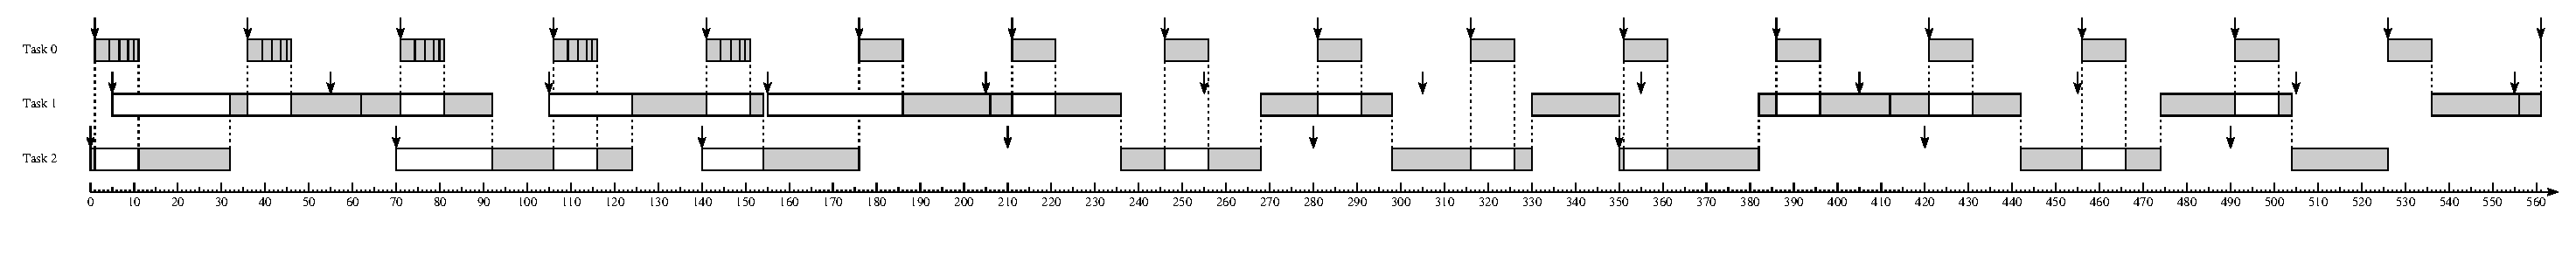
\includegraphics[width=1\linewidth]{figures/multiple_tasks}
	\caption{A timeline for $\mathpzc{T}_{\ref{tab:np_hard}}$ when the set of \textit{extra preemptive} tasks $\mathpzc{E}_i$ is empty. Down-arrows with a "star" denote the activations fo $\tau_d$ that would allow to reduce the response time of $\tau_i$.}
	\label{fig:np_hard1}
\end{figure}

Since the only tasks that can increase the hold time of $\iota_{i,1}$ are the \textit{preemptive} tasks, the problem reduces to find the \textit{preemptive} tasks that minimizes the hold time of  $\iota_{i,1}$ satisfying the constraint $H_{i,1} > 26$. This problem is an instance of the dual of the well known knapsack problem that has been shown to be NP-hard. For task-set $\mathpzc{T}_{\ref{tab:np_hard}}$, the solution of this problem is depicted in Figure \ref{fig:np_hard2}, where the \textit{extra preemptive} tasks that minimize the response time of $\iota_{i,1}$ are $\tau_{h_2}$ and $\tau_{h_3}$. Therefore, the best-case response time of task $\tau_i$ is $BR_i = BC_i+BC_{h2}+BC_{h3} =26.3$.

\begin{figure}[H]
	\centering
	\includegraphics[width=1\linewidth]{figures/multiple_tasks2}
	\caption{A timeline for $\mathpzc{T}_{\ref{tab:np_hard}}$ showing the best-case response time of $\tau_i$ with $BR_i = 26.3$. The set of \textit{extra preemptive} tasks that leads to the best-case response time is $\mathpzc{E}_i=\{\tau_{h_2},\tau_{h_3}\}$.}
	\label{fig:np_hard2}
\end{figure}

\begin{thebibliography}{10}
	\bibitem{BLM13}
	R.J. Bril, J.J. Lukkien, and R.H. Mak.
	Best-case response times and jitter analysis of real-time tasks with arbitrary deadlines.
	In Proc. 21st International Conference on Real-Time Networks and Systems (RTNS), ACM, pp. 193-202, October 2013.
	
\end{thebibliography}


\end{document}

